\appendix

\section{Dataset Construction and Composition}
\label{app:dataset_construction}


\paragraph{AndroidControl\textsuperscript{$\star$} Construction.}
To statically evaluate GUI understanding capability of \METHODNAME beyond
interactive task execution, we construct an extracted AndroidControl
subset, denoted as AndroidControl\textsuperscript{$\star$}. This subset
contains 4,260 step-level records from 781 Android trajectories. Each record
is stored in JSONL format and includes the trajectory identifier, step index,
high-level task goal, per-step instruction, normalized action, screenshot path,
and screenshot resolution. The referenced screenshots are provided as PNG files
and are linked directly from the corresponding step records.

AndroidControl\textsuperscript{$\star$} preserves the same normalized mobile
action space used in \BENCH, including click, scroll, input\_text, open\_app,
wait, navigate\_back, long\_press, and navigate\_home. For actions that can be
matched to a UI element, we also include grounding metadata such as target
bounding boxes, widget class, visible text or content description, resource id,
package name, ancestor information, and the number of matching UI nodes. Steps
without a directly groundable target, such as waiting or app-level operations,
leave the grounding field empty. This subset is mainly used to evaluate static
mobile GUI understanding, verify action-screen alignment, and illustrate the
format of mobile data after normalization.

\paragraph{\BENCH Composition.}

\BENCH is constructed from four groups of trajectories across desktop and
mobile platforms, as summarized in Table~\ref{tab:dataset_composition}. For
each platform, we combine trajectories collected by our Unified
Cross-Platform Data Collection Harness with cleaned open-source
trajectories. On the desktop side, the self-collected portion contains about
95K interaction steps from desktop GUI environments, and the public portion
contains about 13K cleaned steps from OpenCUA~\citep{Opencua}. On the mobile side, the
self-collected portion contains about 17K interaction steps from mobile GUI
environments, and the public portion contains about 35K cleaned steps from
OpenMobile~\citep{openmobile}. In total, \BENCH contains approximately 160K steps and 11.5K
trajectories.

We do not directly use raw public trajectories. Instead, OpenCUA and
OpenMobile are processed with the trajectory cleaning and post-processing
steps described in \cref{app:data_collection_harness}, including
action-space compatibility checking, trajectory filtering, and format
normalization.

\begin{table}[h]
\centering
\caption{Approximate composition of \BENCH. Counts are rounded for readability.}
\label{tab:dataset_composition}
\normalsize
\begin{adjustbox}{max width=\linewidth}
\begin{tabular}{llcc}
\toprule
\textbf{Platform} & \textbf{Source Type} & \textbf{Steps} & \textbf{Trajectories} \\
\midrule
\multirow{2}{*}{Desktop} & Self-collected & $\sim$95K & $\sim$7K \\
 & OpenCUA & $\sim$13K & $\sim$0.8K \\
\multirow{2}{*}{Mobile} & Self-collected & $\sim$17K & $\sim$1K \\
 & OpenMobile & $\sim$35K & $\sim$2.7K \\
\midrule
\multicolumn{2}{l}{Total} & $\sim$160K & $\sim$11.5K \\
\bottomrule
\end{tabular}
\end{adjustbox}
\end{table}

Including OpenCUA and OpenMobile broadens the coverage of GUI states,
applications, and task types beyond the self-collected trajectories. These
sources complement the desktop and mobile data collected by our harness,
increase platform and application diversity, and provide additional
supervision for cross-platform generalization after filtering and
normalization.

\section{Unified Cross-Platform Data Collection Harness}
\label{app:data_collection_harness}

Collecting high-quality GUI agent trajectories is challenging because the
validity of a trajectory depends on the textual instruction, the current
interface state, the executable action space, and the visual grounding of each
interaction. A task that appears reasonable at the language level may still be
unusable for training if the target UI element is not visible, the action
cannot be represented by the student policy, or the instruction is
inconsistent with the environment state. These issues become more pronounced
in a cross-platform setting, where desktop and mobile environments use
different observation formats, action primitives, and UI layouts. To reduce
such noise, the harness organizes data construction into four stages: query generation, 
trajectory collection, trajectory
cleaning, and post-processing.


\begin{figure}[H]
  \centering
  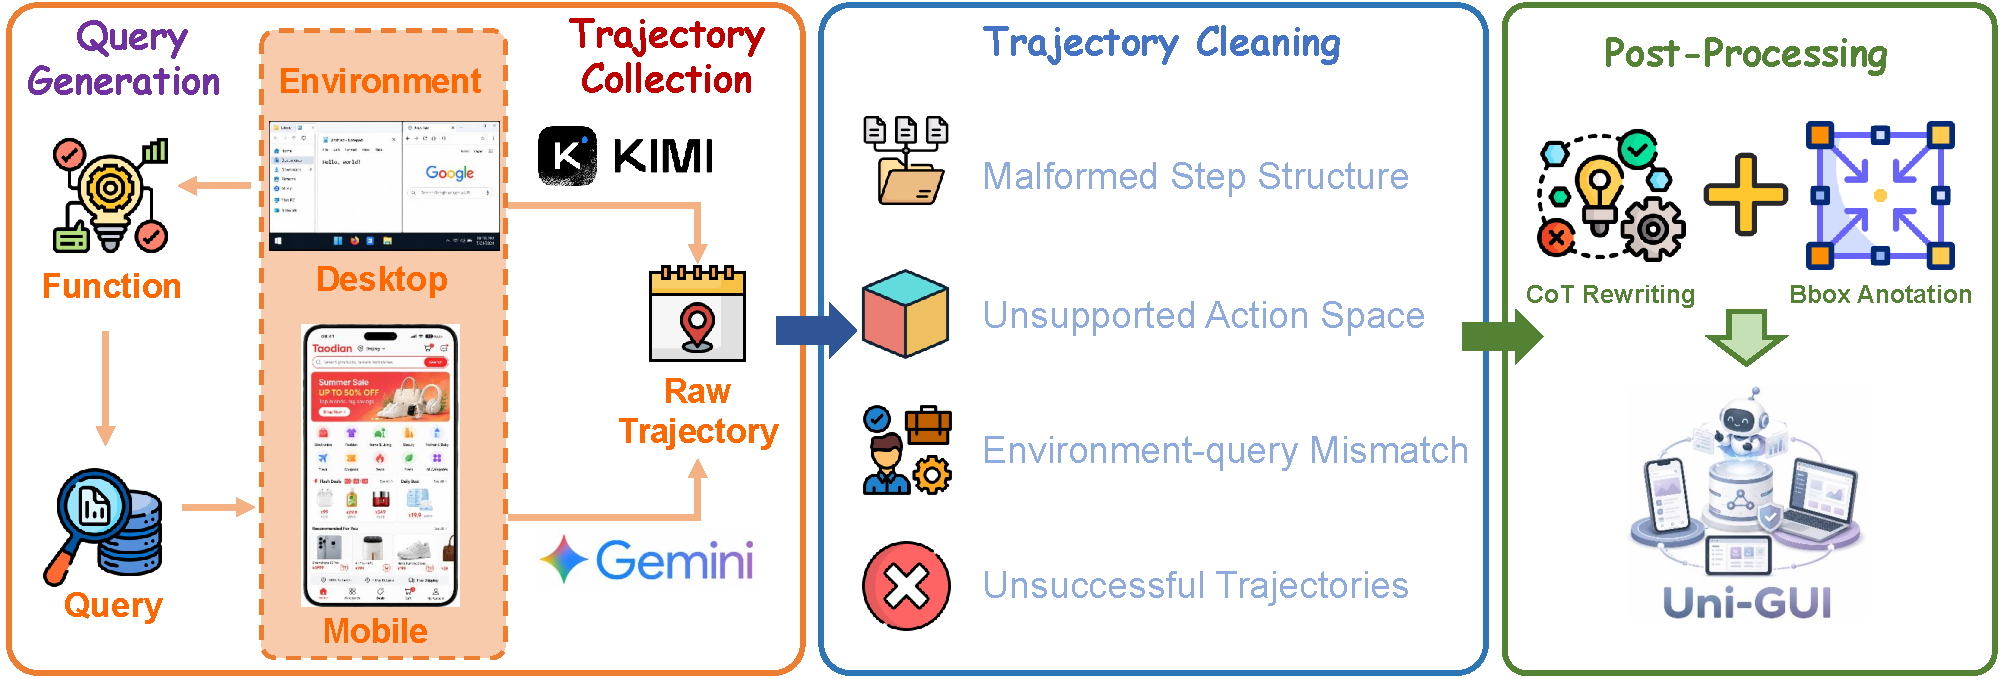
\includegraphics[width=\linewidth]{fig/harness.pdf}
  \caption{Overview of Unified Cross-Platform Data Collection Harness.}
  \label{fig:intro}
\end{figure}


\paragraph{Query Generation.}
We first construct user queries from executable functionalities in the target
environments. Instead of freely generating arbitrary instructions, we ask
strong teacher models to identify realistic functional points supported by the
corresponding desktop or mobile environment, and then synthesize natural user
queries from these functional points. In our implementation, desktop queries
are generated with the assistance of Kimi-K2.6, while mobile queries
are generated with the assistance of Gemini-3.1-Pro. This
environment-grounded query construction reduces the chance of collecting
trajectories for underspecified, infeasible, or state-mismatched tasks.


\paragraph{Query Generation.}
We first construct environment-grounded user queries from real, executable
functionalities in the target GUI environments. For the desktop domain,
Kimi-K2.6 is used to assist functional-point extraction from the
original initialized OSWorld~\citep{osworld} environments. For the mobile domain,
Gemini-3.1-Pro is used to assist functional-point extraction from
the original initialized MobileWorld~\citep{mobileworld} and AndroidWorld~\citep{androidworld} environments. Instead
of generating arbitrary instructions in free form, we ask the teacher models
to identify realistic and usable functionalities supported by these
environments. Based on the extracted functional points, we then synthesize
user queries that are both natural and executable in the corresponding
environments. This design reduces the likelihood of collecting trajectories
for tasks that are underspecified, infeasible, or mismatched with the
environment state.


\paragraph{Trajectory Collection.}
Given a generated query, the teacher model interacts with the target GUI
environment to produce an execution trajectory. Each trajectory records the
observations, actions, intermediate reasoning, and task states during the
rollout. Desktop and mobile trajectories are collected through the same
high-level interface, but the executed actions are kept in their native
platform forms before later normalization. This allows the harness to retain
platform-specific interaction patterns, such as desktop-oriented pointing and
window operations or mobile-oriented touch and navigation behaviors, while
keeping the collected data compatible with a unified training pipeline.

\paragraph{Trajectory Cleaning.}
Raw trajectories collected from GUI environments are noisy and cannot be
directly used for Qwen-VL student-model training. We therefore apply a multi-stage
cleaning pipeline. First, we remove trajectories with malformed step
structures, such as non-contiguous step indices or duplicated steps. Second,
we filter out trajectories whose actions cannot be mapped to the action space
of the student model. This ensures that every retained demonstration can be
faithfully imitated by the student. Third, we discard overly long trajectories
with more than 40 steps, since such trajectories are more likely to contain
inefficient exploration, accumulated errors, or ambiguous supervision signals.
Fourth, we remove trajectories whose queries are inconsistent with the original
environment or unsupported by the collected functional points.


Finally, we use Gemini-3.1-Pro as an automatic judge to check whether the trajectory
successfully completes the intended task, and only retain successful
trajectories. Specifically, we decompose each task query into an
ordered list of sub-tasks before judging. During trajectory inspection, the
judge walks through the execution steps, identifies which sub-task each step
corresponds to, and determines whether the corresponding sub-task has been
completed. A trajectory is retained only when all sub-tasks are judged as
completed. This sub-task-level adjudication avoids relying on a single
long-context judgment over the entire trajectory, reduces the effect of noisy
or redundant steps, and provides clearer attribution for failed executions.



\paragraph{Post-Processing.}
After cleaning, we convert the remaining trajectories into the training format
required by the Qwen-VL-based policy. We first normalize the intermediate
reasoning into a structured chain-of-thought format. This is necessary because
the raw reasoning traces produced by Kimi-K2.6 and
Gemini-3.1-Pro are often heterogeneous in structure, vary
substantially in length, and differ from the reasoning style of Qwen3-VL
models. Directly training on these unnormalized traces may disturb the
student model's original output distribution. Therefore, we rewrite the
reasoning traces into a consistent structure aligned with the expected
Qwen3-VL input-output format.

We also re-annotate grounding bounding boxes for actions that refer to visual
UI elements. These bounding boxes are used in the subsequent rule-based
evaluation stage to determine whether the current action is executed on the
correct target region. The final output of the harness is therefore a set of
successful, executable, action-compatible, reasoning-normalized, and visually
grounded GUI trajectories across both mobile and desktop platforms.




\section{Training and Implementation Details}

\subsection{Action Space and Trajectory Format}

The prompt templates in Appendix~\ref{app:prompt_templates} define the
platform specific tool interfaces used by Qwen3-VL based policies. We
summarize the corresponding action spaces in Table~\ref{tab:action_space}.
Desktop trajectories use the computer\_use interface with
mouse and keyboard actions, while mobile trajectories use the
mobile\_use interface with touchscreen actions. During
post processing, actions from different data sources are converted into these
platform specific tool call formats so that every retained trajectory can be consumed by the training pipeline.

\begin{table}[h]
\centering
\caption{Platform specific action spaces used in the trajectory format.}
\label{tab:action_space}
\normalsize
\setlength{\tabcolsep}{8pt}
\renewcommand{\arraystretch}{1.18}
\begin{tabular}{p{0.11\linewidth}p{0.15\linewidth}p{0.62\linewidth}}
\toprule
\textbf{Platform} & \textbf{Tool} & \textbf{Actions} \\
\midrule
\multirow{2}{*}{Desktop} &
\multirow{2}{*}{computer\_use} &
key, type, mouse\_move, left\_click, left\_click\_drag, right\_click \\
& & middle\_click, double\_click, triple\_click, scroll, wait, terminate \\
\addlinespace[5pt]
\multirow{2}{*}{Mobile} &
\multirow{2}{*}{mobile\_use} &
click, long\_press, swipe, type, answer \\
& & system\_button, wait, ask\_user, terminate \\
\bottomrule
\end{tabular}
\end{table}

Each trajectory is stored as an episode directory. A mobile episode
contains a normalized trajectory file task.json, a raw generation
record task\_raw.json, and screenshots indexed by step, such as
0.jpg and 1.jpg. The normalized
task.json file stores episode metadata, including the task
source, application name, application package, screen resolution, user query,
episode identifier, device type, and train/test split. Its data
field contains the step trajectory records. Each step records the step
index, query, normalized reasoning, tool call action plan, screen resolution,
grounding bounding boxes, screenshot path, and filtering or
review flags.

The raw file task\_raw.json is retained for traceability. It stores
the original prompt, raw model response, raw action, converted action, and
labeled screenshot reference for each step. This separation allows us to keep
the original generation evidence while training only on the cleaned and
normalized trajectory representation.


\subsection{Training Hyperparameters}

Table~\ref{tab:training_hyperparameters} summarizes the main training
configuration used in our experiments. The student policy is initialized from
Qwen3-VL-8B-Thinking, while the platform-specific teachers are
initialized from Qwen3-VL-32B-Thinking. Both teacher SFT and student
training are run for one epoch. Student training uses a GRPO-based DAPO
objective with multi-teacher on-policy distillation, where each prompt samples
8 rollouts and the OPD auxiliary KL loss is enabled with coefficient 0.01.
For visual inputs, training uses only the current screenshot, while inference
uses four historical screenshots, the current screenshot, and the full text
action history.
All training is conducted on 64 NVIDIA H100 GPUs organized as 8 nodes with
8 GPUs each, and asynchronous rollouts are served by SGLang.

\begingroup
\normalsize
\setlength{\tabcolsep}{4pt}
\renewcommand{\arraystretch}{0.96}
\begin{longtable}{lll}
\caption{Training hyperparameters. TP, PP, and DP denote tensor, pipeline, and data parallelism, respectively.}
\label{tab:training_hyperparameters}\\
\toprule
\textbf{Category} & \textbf{Hyperparameter} & \textbf{Value} \\
\midrule
\endfirsthead
\caption[]{Training hyperparameters.}\\
\toprule
\textbf{Category} & \textbf{Hyperparameter} & \textbf{Value} \\
\midrule
\endhead
\bottomrule
\endfoot
\rowcolor{black!8}
\multicolumn{3}{l}{\textit{Models and Training Epochs}} \\
Student model & Initialization & \texttt{Qwen3-VL-8B-Thinking} \\
Teacher model & Initialization & \texttt{Qwen3-VL-32B-Thinking} \\
Teacher SFT & Epochs & 1 \\
Student training & Epochs & 1 \\
\midrule
\rowcolor{black!8}
\multicolumn{3}{l}{\textit{Infrastructure}} \\
Cluster & Nodes / GPUs per node & 8 / 8 \\
Total GPUs & -- & 64 NVIDIA H100 GPUs \\
\midrule
\rowcolor{black!8}
\multicolumn{3}{l}{\textit{Parallelism}} \\
Student 8B & TP / PP / DP & 2 / 1 / 32 \\
Teacher 32B & TP / DP & 8 / 8 \\
Rollout & TP & 2 \\
\midrule
\rowcolor{black!8}
\multicolumn{3}{l}{\textit{Batch Size and Sequence Length}} \\
Training batch size & -- & 128 \\
Generation batch size & -- & 384 \\
Mini batch size & -- & 128 \\
Micro batch size per GPU & -- & 4 \\
Maximum prompt length & -- & 8192 \\
Maximum response length & -- & 512 \\
\midrule
\rowcolor{black!8}
\multicolumn{3}{l}{\textit{Visual Input}} \\
Desktop image resolution & Desktop & $1920 \times 1080$ \\
Mobile image resolution & Mobile & $1080 \times 2400$ \\
Training visual context & Screenshots & Current screenshot only \\
Inference visual context & Screenshots & 4 history screenshots + current screenshot \\
Inference text context & Action history & All previous text actions \\
Image pixel range & Min / max pixels & 3,136 / 13,107,200 \\
\midrule
\rowcolor{black!8}
\multicolumn{3}{l}{\textit{Optimization}} \\
Learning rate & -- & $1\times10^{-6}$ \\
Precision & -- & bfloat16 \\
Rollout samples per prompt & -- & 8 \\
Clip ratio & Low / high / C & 0.2 / 0.28 / 10.0 \\
Loss aggregation & -- & Token mean \\
\midrule
\rowcolor{black!8}
\multicolumn{3}{l}{\textit{OPD KL Loss}} \\
KL loss type & -- & k3 \\
KL loss coefficient & -- & 0.01 \\
\midrule
\rowcolor{black!8}
\multicolumn{3}{l}{\textit{Rollout Engine}} \\
Engine & -- & SGLang \\
Mode & -- & Async \\
Temperature / top-$p$ & -- & 1.0 / 1.0 \\
GPU memory utilization & -- & 0.60 \\
Maximum number of sequences & -- & 1024 \\
\end{longtable}
\endgroup









\section{Fine-Grained Static GUI and Grounding Results}
\label{app:fine_grained_static_grounding}

\begin{table}[H]
\centering
\caption{Fine-grained results on AndroidControl\textsuperscript{$\star$} and grounding benchmarks. AndroidControl\textsuperscript{$\star$} denotes the evaluated subset. Base denotes Qwen3-VL-8B-Thinking, and Model Merge corresponds to the TIES-merging checkpoint.}
\label{tab:appendix_fine_grained_static_grounding}
\normalsize
\setlength{\tabcolsep}{4pt}
\renewcommand{\arraystretch}{0.92}
\begin{adjustbox}{max width=\linewidth}
\begin{tabular}{lccc}
\toprule
\textbf{Benchmark / Metric} & \textbf{Base} & \textbf{Model Merge (TIES)} & \textbf{\METHODNAME} \\
\midrule
\rowcolor{black!8}
\multicolumn{4}{l}{\textit{AndroidControl\textsuperscript{$\star$}}} \\
Action Type Accuracy & 85.75\% & 81.62\% & 87.02\% \\
Grounding (target) & 88.04\% & 86.02\% & 88.33\% \\
Grounding (ancestor) & 89.59\% & 87.69\% & 89.98\% \\
Overall Accuracy & 78.73\% & 74.01\% & 80.05\% \\
\midrule
\rowcolor{black!8}
\multicolumn{4}{l}{\textit{ScreenSpot-Pro}} \\
Overall & 43.71\% & 37.13\% & 43.14\% \\
CAD & 24.90\% & 20.31\% & 22.61\% \\
Dev & 41.81\% & 32.78\% & 41.14\% \\
Creative & 41.06\% & 35.48\% & 41.64\% \\
Scientific & 50.39\% & 50.79\% & 52.36\% \\
Office & 64.78\% & 49.57\% & 63.48\% \\
OS & 42.86\% & 36.73\% & 40.31\% \\
\midrule
\rowcolor{black!8}
\multicolumn{4}{l}{\textit{ScreenSpotV2}} \\
Overall & 91.27\% & 88.60\% & 90.88\% \\
mobile & 93.41\% & 92.02\% & 91.62\% \\
desktop & 90.12\% & 88.02\% & 92.22\% \\
web & 89.70\% & 85.13\% & 89.02\% \\
\midrule
\rowcolor{black!8}
\multicolumn{4}{l}{\textit{OSWorld-G}} \\
Overall & 52.13\% & 47.16\% & 52.84\% \\
Text Matching & 31.58\% & 47.37\% & 42.11\% \\
Element Recognition & 59.70\% & 47.76\% & 57.46\% \\
Layout Understanding & 56.44\% & 53.78\% & 60.44\% \\
Fine-grained Manipulation & 51.52\% & 48.48\% & 50.76\% \\
Refusal & 24.07\% & 14.81\% & 18.52\% \\
\bottomrule
\end{tabular}
\end{adjustbox}
\end{table}

Table~\ref{tab:appendix_fine_grained_static_grounding} provides fine-grained
results for the static GUI and grounding evaluations. On
AndroidControl\textsuperscript{$\star$}, \METHODNAME improves all reported
metrics over the base model, including action type prediction, target
grounding, ancestor grounding, and overall accuracy. In contrast, Model Merge
consistently degrades these metrics, suggesting that static parameter merging
is less stable for preserving mobile GUI understanding.

For the grounding benchmarks, \METHODNAME largely preserves the base model's
performance while avoiding the larger degradation observed in Model Merge.
On ScreenSpot-Pro and ScreenSpotV2, \METHODNAME remains close to the base
model and improves several subcategories such as Creative, Scientific, and
desktop grounding. On OSWorld-G, \METHODNAME achieves the best overall score
and improves layout understanding, indicating that multi-teacher on-policy
distillation can retain fine-grained GUI grounding ability while improving
cross-platform interactive performance.


\section{Additional Case Studies}
\label{sec:exp_case_study2}

Figure~\ref{fig:desktopcase} shows an additional desktop GUI case study. The
example illustrates that \METHODNAME can follow a multi-step desktop
instruction, locate task-relevant regions in a dense interface, and execute
mouse-and-keyboard actions according to the current screen state. Compared
with mobile tasks, desktop tasks require handling larger layouts, window-level
operations, and more precise cursor-based grounding. Together with the mobile
case in Section~\ref{sec:exp_case_study}, this example qualitatively supports
the cross-platform capability of \METHODNAME.

\begin{figure}[H]
  \centering
  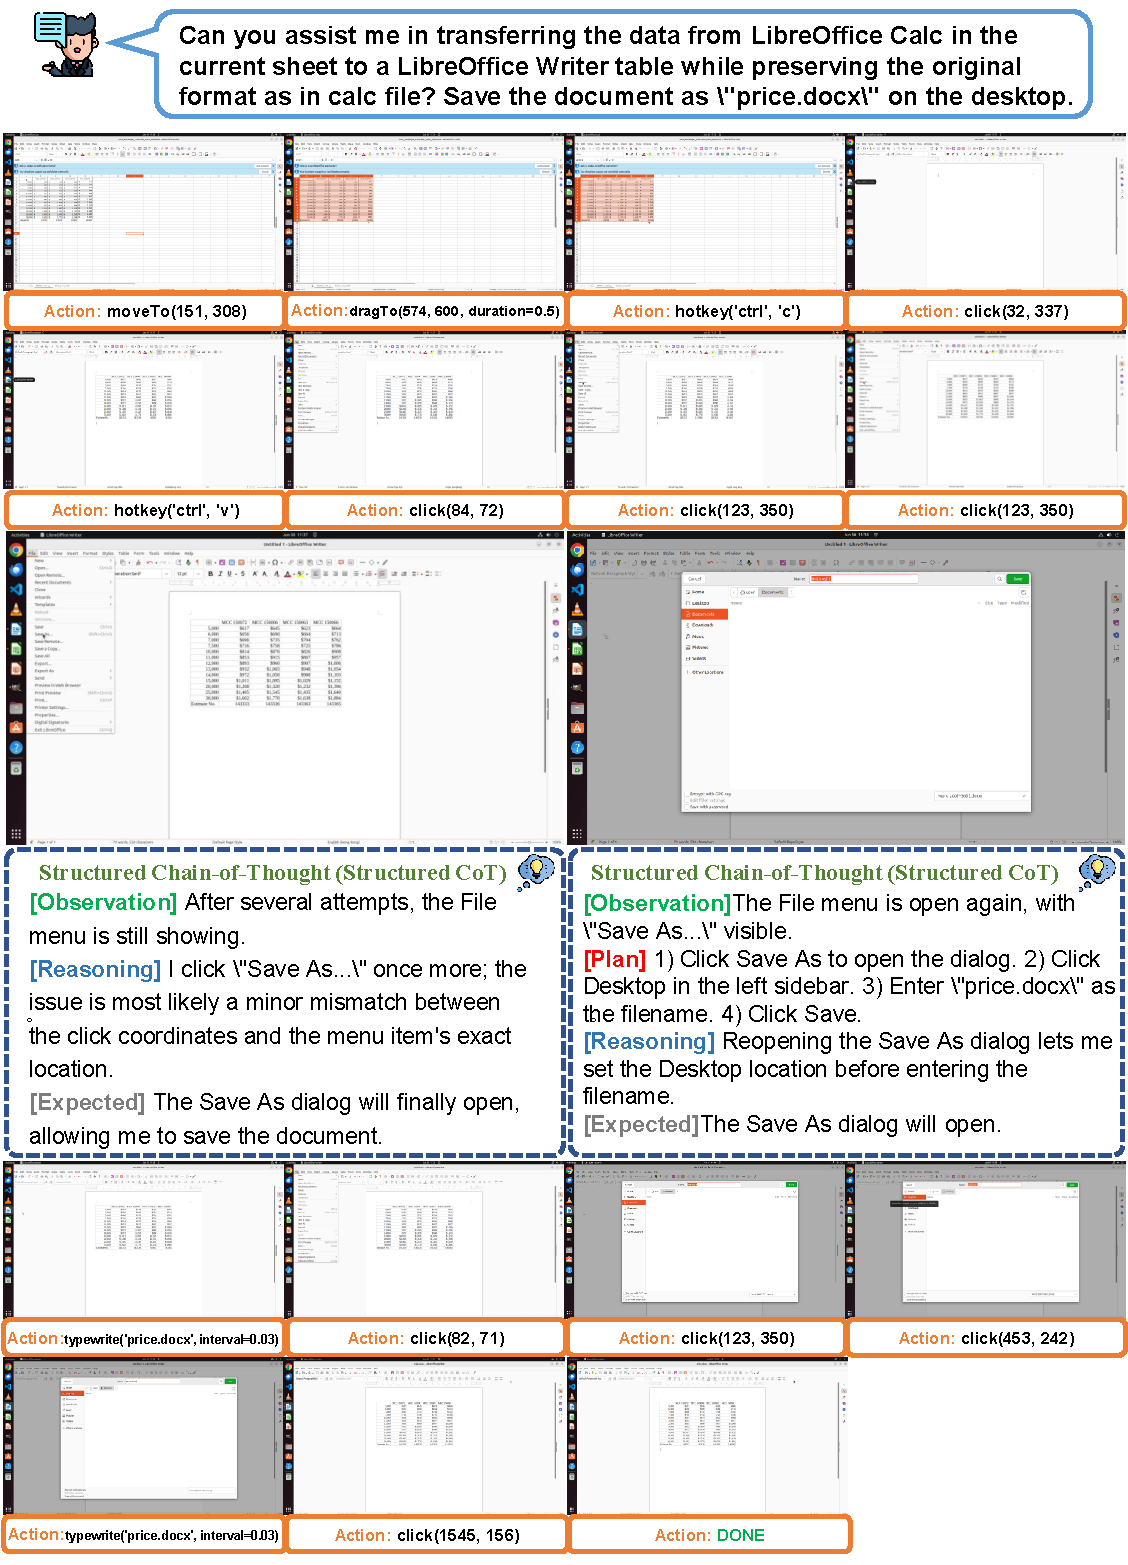
\includegraphics[width=0.90\linewidth]{fig/desktopcase.pdf}
  \caption{Desktop task execution example of \METHODNAME.}
  \label{fig:desktopcase}
\end{figure}

\clearpage
\section{Prompt Templates}
\label{app:prompt_templates}

We provide four system prompts used in our data construction and policy
training pipeline. The first two prompts define the normalized desktop and
mobile tool interfaces for Qwen3-VL-based policies, which are used during
training and evaluation. The other two prompts are used for trajectory
collection: Kimi-K2.6 is used to collect desktop trajectories, while
Gemini-3.1-Pro is used to collect mobile trajectories before action
normalization and post-processing.

\begin{tcblisting}{
  enhanced,
  breakable,
  listing only,
  colback=black!2,
  colframe=xiaomievbg,
  title={Desktop System Prompt (Qwen3-VL)},
  fonttitle=\bfseries,
  arc=1mm,
  boxrule=0.6pt,
  left=1mm,
  right=1mm,
  top=1mm,
  bottom=1mm,
  listing options={
    basicstyle=\ttfamily\footnotesize,
    breaklines=true,
    columns=fullflexible,
    keepspaces=true
  }
}
# Tools

You may call one or more functions to assist with the user query.

You are provided with function signatures within <tools></tools> XML tags:
<tools>
{
  "type": "function",
  "function": {
    "name_for_human": "computer_use",
    "name": "computer_use",
    "description": "Use a mouse and keyboard to interact with a computer, and take screenshots. This is an interface to a desktop GUI. You do not have access to a terminal or applications menu. You must click on desktop icons to start applications. Some applications may take time to start or process actions, so you may need to wait and take successive screenshots. The screen resolution is 1000x1000. Consult screenshots before moving the cursor, and click UI elements with the cursor tip near the center.",
    "parameters": {
      "properties": {
        "action": {
          "enum": ["key", "type", "mouse_move", "left_click", "left_click_drag", "right_click", "middle_click", "double_click", "triple_click", "scroll", "wait", "terminate"]
        },
        "keys": {"description": "Required only by action=key."},
        "text": {"description": "Required only by action=type."},
        "coordinate": {"description": "The x,y coordinates for mouse actions."},
        "pixels": {"description": "The amount of scrolling."},
        "time": {"description": "The seconds to wait."},
        "status": {"enum": ["success", "failure"]}
      },
      "required": ["action"]
    }
  }
}
</tools>

For each function call, return a JSON object with function name and arguments within <tool_call></tool_call> XML tags:
<tool_call>
{"name": <function-name>, "arguments": <args-json-object>}
</tool_call>

# Response format

Response format for every step:
1) Action: a short imperative describing what to do in the UI.
2) A single <tool_call>...</tool_call> block containing only the JSON:
   {"name": <function-name>, "arguments": <args-json-object>}.

Rules:
- Output exactly in the order: Action, <tool_call>.
- Be brief: one sentence for Action.
- Do not output anything else outside those parts.
- If finishing, use action=terminate in the tool call.
\end{tcblisting}

\clearpage
\begin{tcblisting}{
  enhanced,
  breakable,
  listing only,
  colback=black!2,
  colframe=xiaomievbg,
  title={Mobile System Prompt (Qwen3-VL)},
  fonttitle=\bfseries,
  arc=1mm,
  boxrule=0.6pt,
  left=1mm,
  right=1mm,
  top=1mm,
  bottom=1mm,
  listing options={
    basicstyle=\ttfamily\footnotesize,
    breaklines=true,
    columns=fullflexible,
    keepspaces=true
  }
}
# Tools

You may call one or more functions to assist with the user query.

You are provided with function signatures within <tools></tools> XML tags:
<tools>
{
  "type": "function",
  "function": {
    "name": "mobile_use",
    "description": "Use a touchscreen to interact with a mobile device, and take screenshots. This is an interface to a mobile device with touchscreen. You can perform actions like clicking, typing, swiping, etc. Some applications may take time to start or process actions, so you may need to wait and take successive screenshots. The screen resolution is 999x999. Click buttons, links, and icons near the center of the element.",
    "parameters": {
      "properties": {
        "action": {
          "enum": ["click", "long_press", "swipe", "type", "answer", "system_button", "wait", "ask_user", "terminate"]
        },
        "coordinate": {"description": "Required only by action=click, action=long_press, and action=swipe."},
        "coordinate2": {"description": "Required only by action=swipe."},
        "text": {"description": "Required only by action=type, action=ask_user, and action=answer."},
        "time": {"description": "Required only by action=long_press and action=wait."},
        "button": {"enum": ["Back", "Home", "Menu", "Enter"]},
        "status": {"enum": ["success", "failure"]}
      },
      "required": ["action"]
    }
  }
}
</tools>

For each function call, return a JSON object with function name and arguments within <tool_call></tool_call> XML tags:
<tool_call>
{"name": <function-name>, "arguments": <args-json-object>}
</tool_call>

# Response format

Response format for every step:
1) Thought: one concise sentence explaining the next move.
2) Action: a short imperative describing what to do.
3) A single <tool_call>...</tool_call> block containing only the JSON:
   {"name": <function-name>, "arguments": <args-json-object>}.

Rules:
- Output exactly in the order: Thought, Action, <tool_call>.
- Be brief: one sentence for Thought, one sentence for Action.
- Do not output anything else outside those three parts.
- If finishing, use mobile_use with action=terminate in the tool call.
\end{tcblisting}

\clearpage
\begin{tcblisting}{
  enhanced,
  breakable,
  listing only,
  colback=black!2,
  colframe=black!85,
  colbacktitle=black!85,
  coltitle=white,
  title={Desktop Trajectory Collection Prompt (Kimi-K2.6)},
  fonttitle=\bfseries,
  arc=1mm,
  boxrule=0.6pt,
  left=1mm,
  right=1mm,
  top=1mm,
  bottom=1mm,
  listing options={
    basicstyle=\ttfamily\footnotesize,
    breaklines=true,
    columns=fullflexible,
    keepspaces=true
  }
}
System Prompt

You are a GUI agent. You are given an instruction, a screenshot of the screen,
and your previous interactions with the computer. You need to perform a series
of actions to complete the task. The password of the computer is {password}.

For each step, provide your response in this format:
{thought}
## Action:
{action}
## Code:
{code}

In the code section, the code should be either pyautogui code or one of the
following functions wrapped in the code block:

- {
    "name": "computer.wait",
    "description": "Make the computer wait for 20 seconds for installation,
    running code, etc.",
    "parameters": {
      "type": "object",
      "properties": {},
      "required": []
    }
  }

- {
    "name": "computer.terminate",
    "description": "Terminate the current task and report its completion status",
    "parameters": {
      "type": "object",
      "properties": {
        "status": {
          "type": "string",
          "enum": ["success", "failure"],
          "description": "The status of the task"
        },
        "answer": {
          "type": "string",
          "description": "The answer of the task"
        }
      },
      "required": ["status"]
    }
  }
\end{tcblisting}

\clearpage
\begin{tcblisting}{
  enhanced,
  breakable,
  listing only,
  colback=blue!2!violet!3,
  colframe=blue!45!violet!85!black,
  colbacktitle=blue!45!violet!85!black,
  coltitle=white,
  title={Mobile Trajectory Collection Prompt (Gemini-3.1-Pro)},
  fonttitle=\bfseries,
  arc=1mm,
  boxrule=0.6pt,
  left=1mm,
  right=1mm,
  top=1mm,
  bottom=1mm,
  listing options={
    basicstyle=\ttfamily\footnotesize,
    breaklines=true,
    columns=fullflexible,
    keepspaces=true
  }
}
# Role: Android Phone Operator AI

You are an AI that controls an Android phone to complete user requests.
Your responsibilities:
- Answer questions by retrieving information from the phone.
- Perform tasks by executing precise actions.

# Action Framework

Respond with exact JSON format for one of these actions:
| Action | Description | JSON Format Example |
| click | Tap visible element | {"action_type": "click", "coordinate": [x, y]} |
| double_tap | Double tap visible element | {"action_type": "double_tap", "coordinate": [x, y]} |
| long_press | Long press visible element | {"action_type": "long_press", "coordinate": [x, y]} |
| drag | Drag from one visible element to another | {"action_type": "drag", "start_coordinate": [x1, y1], "end_coordinate": [x2, y2]} |
| input_text | Type into field | {"action_type": "input_text", "text": "Hello"} |
| answer | Respond to user | {"action_type": "answer", "text": "It's 25 degrees today."} |
| navigate_home | Return to home screen | {"action_type": "navigate_home"} |
| navigate_back | Navigate back | {"action_type": "navigate_back"} |
| scroll | Scroll direction | {"action_type": "scroll", "direction": "down"} |
| status | Mark task as complete or infeasible | {"action_type": "status", "goal_status": "complete"} |
| wait | Wait for screen to update | {"action_type": "wait"} |
| ask_user | Ask user for information | {"action_type": "ask_user", "text": "what is the exact requirements do you need?"} |
| keyboard_enter | Press enter key | {"action_type": "keyboard_enter"} |
Note:
- The coordinate is the center of the element to be clicked, long pressed, or dragged.
- x and y are screen coordinates, with origin at the top left corner.
- x and y are normalized to [0, 1000].
# Execution Principles
1. Communication Rule:
- Always use the answer action to reply to users.
- Follow the user instruction strictly, e.g., only return a single number,
  only return True or False, or only return items separated by comma.
- Never use answer to indicate waiting or loading; use wait instead.
- The answer action terminates the task immediately.
2. Efficiency First:
- Choose the simplest path to complete tasks.
- If an action fails twice, try alternatives, e.g., long_press instead of click.
3. Smart Navigation:
- Gather information when needed.
- For scrolling, scroll direction is inverse to swipe direction.
- If scroll fails, try the opposite direction.
4. Text Operations:
- First click the input box to activate it before typing.
- For text manipulation, long press to select, use selection bar options,
  and delete by selecting then cutting.
5. Ask User:
- If there is not enough information to complete the task, use ask_user.
# Decision Process
1. Analyze goal, history, and current screen.
2. Determine if the task is already complete, and use status if true.
3. If not, choose the most appropriate action.
4. Output in the exact format below. The action must be a valid JSON string.
5. Only one tool call is allowed in one action.
# Expected Output Format

Thought: [Analysis including reference to key steps or points when applicable]
Action: [Single JSON action]

# Output Format Example
Thought: I need to type the weather question into the search box.
Action: {"action_type": "input_text", "text": "What is weather like in San Francisco today?"}
\end{tcblisting}
